\documentclass[../../../../main.tex]{subfiles}

\begin{document}

\section*{東大理科数学 1990年}

やって来ました 90年代!

\begin{center}
\begin{tabular}{|c|c|c|c|c|}
\hline
 & 分野 & 計 & 見 & 統 \\ \hline
1 & 単純な極限 & A & B & B \\ \hline
2 & 3次関数の性質 & B & C & C \\ \hline
3 & 空間 & C & C & C \\ \hline
4 & 行列 & & & \\ \hline
5 & 多変数-双曲線 & C & C & C \\ \hline
6 & 場合の数- & C & D & D \\ \hline
\end{tabular}
\end{center}

\newpage

\subsection*{第1問}

\begin{center}
\begin{framed}
$a_n = \displaystyle\sum_{k=1}^n \frac{1}{\sqrt{k}}$, $b_n = \displaystyle\sum_{k=1}^n \frac{1}{\sqrt{2k+1}}$ として

$a_n, \quad \frac{b_n}{a_n} \to ? \quad (n \to \infty)$
\end{framed}
\end{center}

\noindent
\textbf{[解]} $\sum_{k=1}^n f(k)$ は下図斜線部の面積を表す。

\begin{center}
\begin{tikzpicture}[scale=1.5, >=stealth]
  % Upper graph
  \draw[->] (-0.2,0) -- (3.5,0) node[right] {$x$};
  \draw[->] (0,-0.2) -- (0,2.2) node[above] {$y$};
  \node[below left] at (0,0) {$O$};

  \draw[thick, domain=0.4:3.2, samples=50] plot (\x, {1/sqrt(\x)}) node[right] {$y=f(x)$};

  \fill[pattern=north east lines, pattern color=gray!60] (0.5,0) rectangle (1, {1/sqrt(0.5)});
  \draw (0.5,0) -- (0.5, {1/sqrt(0.5)}) -- (1, {1/sqrt(0.5)}) -- (1,0);
  
  \fill[pattern=north east lines, pattern color=gray!60] (2.2,0) rectangle (2.7, {1/sqrt(2.2)});
  \draw (2.2,0) -- (2.2, {1/sqrt(2.2)}) -- (2.7, {1/sqrt(2.2)}) -- (2.7,0);

  \draw (1,0) node[below] {$1$};
  \draw (2.7,0) node[below] {$n$};
\end{tikzpicture}
\quad
\begin{tikzpicture}[scale=1.5, >=stealth]
  % Lower graph
  \draw[->] (-0.2,0) -- (3.5,0) node[right] {$x$};
  \draw[->] (0,-0.2) -- (0,2.2) node[above] {$y$};
  \node[below left] at (0,0) {$O$};

  \draw[thick, domain=0.4:3.2, samples=50] plot (\x, {1/sqrt(\x)}) node[right] {$y=f(x)$};

  \fill[pattern=north east lines, pattern color=gray!60] (1,0) rectangle (1.5, {1/sqrt(1.5)});
  \draw (1,0) -- (1, {1/sqrt(1.5)}) -- (1.5, {1/sqrt(1.5)}) -- (1.5,0);

  \fill[pattern=north east lines, pattern color=gray!60] (2.2,0) rectangle (2.7, {1/sqrt(2.7)});
  \draw (2.2,0) -- (2.2, {1/sqrt(2.7)}) -- (2.7, {1/sqrt(2.7)}) -- (2.7,0);

  \draw (1,0) node[below] {$1$};
  \draw (2.2,0) node[below] {$n$};
  \draw (2.7,0) node[below] {$n+1$};
\end{tikzpicture}
\end{center}

\noindent
従って面積を比較して,
\[
\int_1^n \frac{1}{\sqrt{x}} \, dx + \frac{1}{\sqrt{n+1}} < a_n < \int_1^n \frac{1}{\sqrt{x}} \, dx + 1
\]
\[
\frac{1}{\sqrt{2}} \int_1^n \frac{1}{\sqrt{x + 1/2}} \, dx + \frac{1}{\sqrt{2n+3}} < b_n < \frac{1}{\sqrt{2}} \int_1^n \frac{1}{\sqrt{x + 1/2}} \, dx + \frac{1}{\sqrt{3}}
\]
だから, 計算して,
\[
2\sqrt{n} + \frac{1}{\sqrt{n+1}} - 2 < a_n < 2\sqrt{n} - 1 \quad \dots \text{①}
\]
\[
\sqrt{2n+1} + \frac{1}{\sqrt{2n+3}} - \sqrt{3} < b_n < \sqrt{2n+1} \quad \dots \text{②}
\]
①は, 最左辺, 右辺共に $+\infty$ に発散するので, はさみうちより
\[
a_n \to +\infty \quad (n \to \infty)
\]
$n \to \infty$ を考えるので, ①, ②は共に各辺正として良く,
\[
\frac{\sqrt{2n+1} - \sqrt{3} + \frac{1}{\sqrt{2n+3}}}{2\sqrt{n}-1} < \frac{b_n}{a_n} < \frac{\sqrt{2n+1}}{2\sqrt{n} + \frac{1}{\sqrt{n+1}} - 2}
\]
\[
\frac{\sqrt{2 + 1/n} - \sqrt{3/n} + \frac{1}{\sqrt{n(2n+3)}}}{2 - 1/\sqrt{n}} < \frac{b_n}{a_n} < \frac{\sqrt{2 + 1/n}}{2 - 2/\sqrt{n} + \frac{1}{\sqrt{(n+1)n}}}
\]
両辺共に $n \to \infty$ で $\frac{1}{\sqrt{2}}$ に収束するので, はさみうちより
\[
\frac{b_n}{a_n} \to \frac{1}{\sqrt{2}} \quad (n \to \infty)
\]

\newpage

\subsection*{第2問}

\begin{center}
\begin{framed}
3次関数 $h(x) = px^3 + qx^2 + rx + s$ が次をみたす.
\begin{enumerate}[(i)]
    \item $h(1) = 1, \, h(-1) = -1$
    \item $(-1, 1)$ で極値 $\pm 1$ を取る.
\end{enumerate}
この時,
\begin{enumerate}[(1)]
    \item $h(x) = ??$
    \item 3次関数 $f(x) = ax^3 + bx^2 + cx + d$ が $(-1, 1)$ で $-1 < f(x) < 1$ をみたす時, $|x| > 1$ なる任意の $x$ で $|f(x)| < |h(x)|$ であることを示せ.
\end{enumerate}
\end{framed}
\end{center}

\noindent
$\rhd$ まず, 前半の関数決定について.
\begin{itemize}
    \item 極値を用いて $f'(x)$ を表す.
    \item 因数定理で因数分解
\end{itemize}
特に3次は, $f'(x)$ の回解形から, 極値での因数分解が有効である. ($\alpha, \beta$ がわかる状態であるので)

\begin{center}
\begin{framed}
\textbf{[解答例1]}

$\begin{cases}
h(x) - 1 = A(x-\alpha)^2 (x-1) \\
h(x) + 1 = B(x-\beta)^2 (x+1)
\end{cases}$ \quad ($\alpha, \beta$ で極値をとる)

とおいて, 係数比較
\end{framed}
\end{center}

\noindent
$\rhd$ グラフをかくと $-1 \le x \le 1$ に必ず3交点を持つから, 
\[
\text{$n$次関数の交点は高々$n$個}
\]
を使えそう.

$\to$ こまかい場合分けは\dots
\begin{enumerate}[(1)]
    \item $-1 \le x \le 1$ で $|f(x)| < 1$ なら OK
    \item 例えば $f(1) = -1$ なら, 下のようなことがある.
\end{enumerate}
$\to$ そこで定量的にやった方がラクそう.

\noindent
$\rhd$ そこで, $f(x) = h(x) + k(x-\alpha)(x-\beta)(x-t)$ とおく. $k$ の符号次第で $|x| > 1$ で符号一定だから $f, h$ の大小がキマル.

たとえば $x = 1/2$ では, $h(1/2) = -1 < f(1/2)$ から, $k$ の正負がわかってオワリ.

\vspace{1em}

\noindent
\textbf{[解]}
(1) $-1 < x < 1$ で $h(x)$ が極値をとる $x$ を $\alpha, \beta$ とおくと,
\begin{align}
h(x) - 1 &= p(x-1)(x-\alpha)^2 \quad \dots \text{①} \\
h(x) + 1 &= p(x+1)(x-\beta)^2 \quad \dots \text{②}
\end{align}
だから
\[
h'(x) = p(x-\alpha)^2 + 2p(x-1)(x-\alpha) = p(x-\alpha)(3x - \alpha - 2)
\]
となり, $\beta = \frac{\alpha+2}{3}$ である。②に代入して
\[
h(x) + 1 = p(x+1)\left(x - \frac{\alpha+2}{3}\right)^2
\]
①, ②で係数比較して,
\[
2\text{次} \dots p\left(1 - \frac{2\alpha+4}{3}\right) = p(-1-2\alpha)
\]
から $p \neq 0$ より $\alpha = -\frac{1}{2}$. 定数項を比較して,
\[
1 - \frac{1}{4}p = -1 + \frac{4}{9}p \quad \dots \quad \therefore p = 4
\]
①に代入して
\[
h(x) = 4(x-1)\left(x + \frac{1}{2}\right)^2 + 1 = 4x^3 - 3x_{\#}
\]

\noindent
(2)
\begin{center}
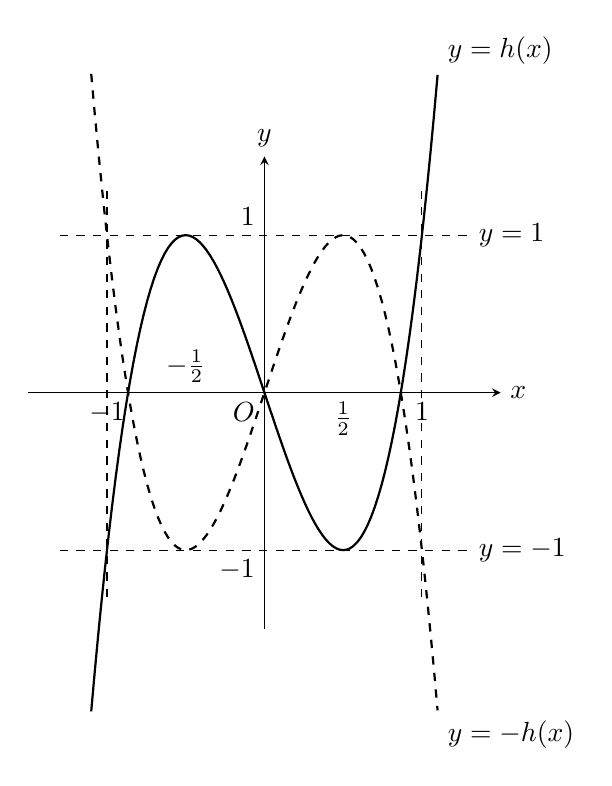
\begin{tikzpicture}[scale=2, >=stealth]
  % Axes
  \draw[->] (-1.5,0) -- (1.5,0) node[right] {$x$};
  \draw[->] (0,-1.5) -- (0,1.5) node[above] {$y$};
  \node[below left] at (0,0) {$O$};

  % Dashed lines y = 1, y = -1
  \draw[dashed] (-1.3,1) -- (1.3,1) node[right] {$y=1$};
  \draw[dashed] (-1.3,-1) -- (1.3,-1) node[right] {$y=-1$};

  % Dashed vertical lines x = 1, x = -1
  \draw[dashed] (1,-1.3) -- (1,1.3);
  \draw[dashed] (-1,-1.3) -- (-1,1.3);

  % Labels on axes
  \node[above left] at (0,1) {$1$};
  \node[below left] at (0,-1) {$-1$};
  \node[below] at (1,0) {$1$};
  \node[below] at (-1,0) {$-1$};
  \node[below] at (0.5,0) {$\frac{1}{2}$};
  \node[above] at (-0.5,0) {$-\frac{1}{2}$};

  % Curve y = h(x) = 4x^3 - 3x
  \draw[thick, domain=-1.1:1.1, samples=100] plot (\x, {4*\x*\x*\x - 3*\x}) node[above right] {$y=h(x)$};

  % Curve y = -h(x)
  \draw[dashed, thick, domain=-1.1:1.1, samples=100] plot (\x, {-(4*\x*\x*\x - 3*\x)}) node[below right] {$y=-h(x)$};
\end{tikzpicture}
\end{center}

$y=f(x), h(x)$ は連続な関数で, $h(-1)=-1, h(-1/2)=1, h(1/2)=-1, h(1)=1$ から, この2関数は $-1 < x < -\frac{1}{2}, \, -\frac{1}{2} < x < \frac{1}{2}, \, \frac{1}{2} < x < 1$ で交わる。$f, h$ は3次関数だから, $g(x) = f(x) - h(x)$ と定めると, 適当な $0$ でない定数 $k$ と, $-1 < \alpha < -\frac{1}{2} < \beta < \frac{1}{2} < \gamma < 1$ をみたす $\alpha, \beta, \gamma$ において
\[
g(x) = k(x-\alpha)(x-\beta)(x-\gamma)
\]
とおける。ここで, $g(1/2) = f(1/2) + 1 > 0$, $(1/2-\alpha)(1/2-\beta)(1/2-\gamma) < 0$ から, $k < 0$ である。

したがって,
\[
\begin{cases}
1 < x \text{ においては}, g(x) < 0 \\
x < -1 \quad \text{〃} \quad , g(x) > 0
\end{cases}
\iff
\begin{cases}
1 < x \text{ の時}, h(x) > f(x) \\
x < -1 \text{ の時}, h(x) < f(x)
\end{cases}
\quad \dots \text{①}
\]

$P(x) = f(x) + h(x)$ についても同様の論から,
\[
\begin{cases}
1 < x \text{ の時}, -h(x) < f(x) \\
x < -1 \text{ の時}, f(x) < -h(x)
\end{cases}
\quad \dots \text{②}
\]

①, ②から,
\[
|x| > 1 \text{ の時 } |f(x)| < |h(x)|
\]
である。

\end{document}
